\section{Observations and models}

\subsection{Selection of observations}
We conduct our survey on 138 images taken by the Cassini Image Sub-System Narrow Angle Camera (ISS/NAC) with the
ultra-violet (CL1-UV3) filters. We choose the best possible sample among the 317 images available on the PDS to get the
highest temporal and phase coverage. We kept only images taken with at least one day apart. However, we also considered
specific sets of observations made few hours apart to study short term variations. For the seasonal survey, the average
time between two pictures is 39 Earth days, \textit{i.e.} 2.5 Titan days (Fig.~\ref{fig:img_sampling}). Even if
our sampling is not evenly distributed, due to orbital constraints and mission schedule, at least 90\% of the selected
images are separated by less than 120 Earth days, \textit{i.e.} 7.5 Titan days. There are two time  gaps in our
sample between 28 March 2008 and 25 January 2009 (302 days) and 26 November 2010 and 9 September 2011 (286 days).

\begin{figure}[!ht]
\centering
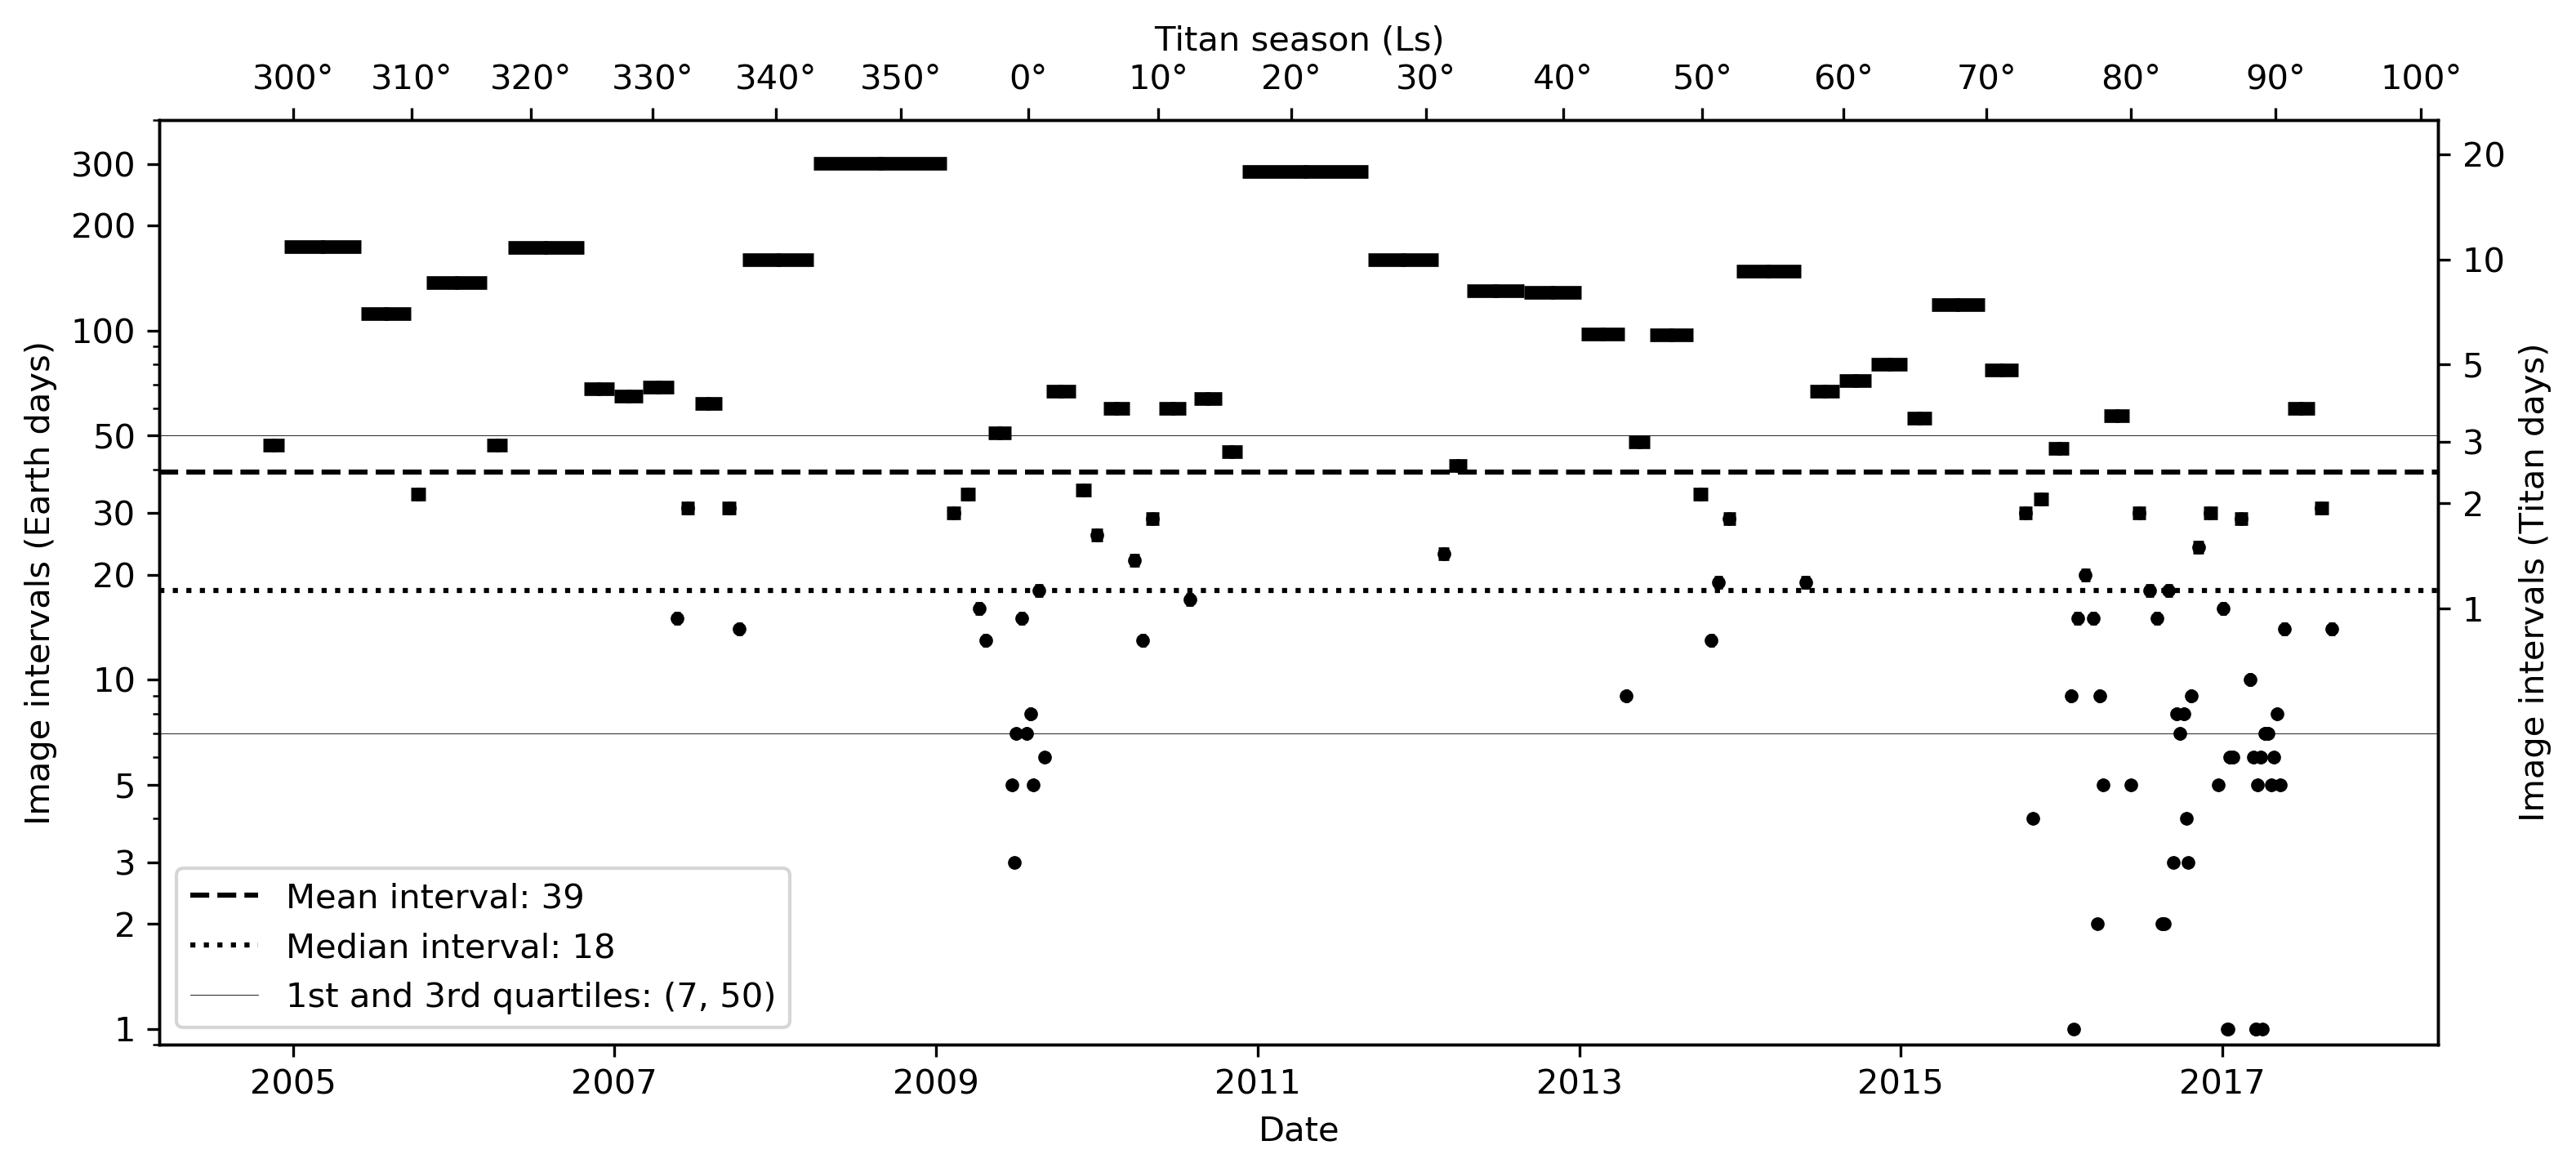
\includegraphics[width=\textwidth]{Fig/IMG_interval.png}
\caption{Image intervals (in Earth and Titan days) between consecutive ISS/NAC CL1-UV3 observations analyzed. On average
an image is sampled every 39 days.}
\label{fig:img_sampling}
\end{figure}

The selected images are calibrated using the CISSCAL routines (v3.8) provided on the Planetary Data System. To improve
the signal to noise ratio on the limb profile, we deconvolved the images with a Poisson Maximum a posteriori method
(PMAP) using the point spread function (PSF) calculated in-flight \citep{West2010}. The image navigation are
initialized with the spice kernel routines and the location of the center of Titan is refined by searching the maximum
of flatness at iso-incident on the limb.

The intensity profiles are extracted every \ang{5} bins, on both sides of the limb. Depending on the location of the
latitude of the Sub-Cassini point on the ground, the sampling in latitude is not evenly distributed for each image.
Geometrically, the polar latitudes are less covered than the equator. The illumination also change drastically during the
season between the northern mid-winter to summer, which restricts our ability to see both poles at the same time.



\subsection{Model of scattering at the limb}

To retrieve the haze extinction profiles from the I/F observations, we first model the synthetic radiance factor ($I/F$)
with a single scattering ray tracing model in a spherical shell geometry. The effect of the multiple scattering is
accounted as a correction with a factor $\varrho_k\left(z\right)$ applied to the volume scattering along line of sight.
This technique was used successfully several time before \citep[e.g.][]{Rages1983, Rannou1997, Seignovert2017, West2018}.

In the detached layer, the multiple scattering is mainly produced by the light coming from the atmosphere below. To
evaluate $\varrho_k$, the scattering properties of the atmosphere are fixed once for all with a setup that allows to
reproduce the observed intensity of Titan in UV. With the radiative transfer model \citep[the SHDOMPP from][]{Evans1998}
we have access to the complete radiative source function at each level of the atmosphere. We are then able to compare the
intensity that is scattered in the direction of the observer from the direct sun only and from the direct sun and the diffuse
field coming from below. $\varrho_k$ is defined as the ratio of multiple scattering to single scattering toward the observer
for a given altitude and as a function of the incident and emergent angles. It is then calculated as a function the
altitude, the incident angle and the emergent angle and set in a look-up table \citep{West2018}.

We discretize the atmosphere in $N=60$ irregular layers of various thickness : $\Delta z =$ 50 km from the
ground to 200 km, $\Delta z =$ 10 km from 300 to 400 km and from 550 to 700 km. Finally, we used
$\Delta z$= 5 km between 400 and 550 km. This grid allows us to fully take advantage of the spatial resolution
of the ISS NAC camera in the region of interest, where is the DHL. We write the outgoing radiance factor $I/F\ (z)$ as:

\begin{equation}
I/F\ (z) = \sum_{i=0}^{n_x-1} \int\limits_{x_k}^{x_{k+1}}
\frac{\left< \varpi P(\Theta) \right>_k} {4}
^{-\left( \tau^i_k\left(z\right) + \tau^e_k\left(z\right) \right)}
\beta_k\left(z\right) \varrho_k\left(z\right) d{x}
\label{eq:west2017_sup_limb}
\end{equation}

where the summation is performed on the $n_x-1$ segments defined by the intersections of the line of sight and the
spherical shells boundaries. The impact factor $z$ (the lowest altitude reached by the line of sight) is given by the
bottom of the $n^\mathrm{th}$ layer crossed. Therefore, each layer of the atmosphere is crossed twice. $x$ is the
abscissa along the line of sight. $\tau^i_k$ and $\tau^e_k$ are the opacities along the incident and emergent paths.
$\left< \varpi P(\Theta)\right>_k$ is the average of the product between the single scattering and the phase function
at the scattering angle of the observation $\Theta$ for the layer crossed on $x_k$.  $\beta_k(z)$ is the local
extinction at the altitude $z$. Here, the altitude $z(x)$ is the local altitude at point of abscissa $x$ along the
line of sight. The correction factor $\varrho_k\left(z\right)$ enhances the volume scattering along the line of sight.
We find that the multiple scattering increases the scattered intensity at the limb of Titan in UV by a ratio between
1.05 and 1.15, depending on the geometry of the observation.


\subsection{Retrieval method}

Based on our previous works \citep{Seignovert2017, West2018}, we make the assumption that the optical properties
$\left<\varpi P(\Theta)\right>_k$ of the aerosols are constant in the upper part of Titan's atmosphere. This allows
us to focus our study only on the retrieval of the extinction along the line of sight.
% We will verify that this assumption is reasonable compared to the dynamical variability observed along the season.

In our model, an $I/F(z)$ profile only depends on the set haze extinction profile $\beta(z)$ on the geometry of
the observation (illumination, viewing and phase angles). We assume no horizontal inhomogeneity in the atmosphere
properties along the line of sight \citep{Seignovert2017}. We retrieve a set of extinction values $\beta_i$ (composing
the vector ${\beta}$), with $i$ the indices of the layers, that matches the values of the radiance factor, $I/F_i$
(composing the vector $I/F$).

From the Eq. (\ref{eq:west2017_sup_limb}), it is possible to cast the scattered intensity $I/F_i$, as a function of
the extinction $\beta_j$ with $j \le i$. This forms a non-linear triangular system. To find the vector $\beta$, we
have to solve the formal equation:

\begin{equation}
    I/F = G(\beta)
\end{equation}

where the ${G}$ is a nonlinear function which depends on the values $\beta_i$ and on the geometry of the observation.
We could solve this system with a standard onion peeling technique and accounting for the error due to the observation
and to the propagation of error caused, at a given level, by the errors on the $\beta_j$ in the layers above ($j<i$).
Instead, we decided to solve the system by minimizing the difference between the modelled  $I/F$ and the observations
using a Levenberg-Marquardt minimization. We then retrieve simultaneously all the values $\beta_i$, but only the layers $i$
for which the tangential opacity along a line of sight ($\tau_{los}$) is small enough have an influence on the value
of $I/F_i$. When $\tau_{los}$ exceeds 3, we consider that the atmosphere is too opaque and beyond this threshold we
do not retrieve the value of $\beta$.
